\subsection{Contexto y objetivo}\label{contexto-y-objetivo}

\begin{frame}{Universidad de Cuenca, DEET, Maestria en Ciencias de la
Ingenieria Electrica}
\protect\phantomsection\label{universidad-de-cuenca-deet-maestria-en-ciencias-de-la-ingenieria-electrica}
Este proyecto aplica teoria de grafos a ciberseguridad: detectar nodos
criticos, modelar propagacion de malware y evaluar resiliencia
topologica.
\end{frame}

\begin{frame}{Objetivo general}
\protect\phantomsection\label{objetivo-general}
\begin{itemize}
\tightlist
\item
  Modelar la red como grafo.
\item
  Calcular metricas de centralidad.
\item
  Detectar anomalias con score compuesto y z-score.
\item
  Simular propagacion de malware con SIR.
\item
  Evaluar resiliencia con articulaciones y puentes.
\item
  Validar con trafico real del dataset IoT-23.
\end{itemize}
\end{frame}

\subsection{Enunciado del problema}\label{enunciado-del-problema}

\begin{frame}{Problema a resolver}
\protect\phantomsection\label{problema-a-resolver}
Procedimiento reproducible para detectar nodos anomalos, priorizar
activos criticos y evaluar respuesta ante propagacion de malware.
\end{frame}

\begin{frame}{Escenario de trabajo}
\protect\phantomsection\label{escenario-de-trabajo}
\begin{itemize}
\tightlist
\item
  \textbf{Escenario 1} (controlado): red corporativa como grafo
  ponderado.
\item
  \textbf{Escenario 2} (real): capturas IoT-23 con etiquetas
  benigno/malicioso.
\item
  \textbf{Resultado esperado}: identificar nodos/IPs de alto riesgo con
  criterio cuantitativo.
\end{itemize}
\end{frame}

\subsection{Procedimiento (paso a
paso)}\label{procedimiento-paso-a-paso}

\begin{frame}[fragile]{Flujo de implementacion}
\protect\phantomsection\label{flujo-de-implementacion}
\begin{enumerate}
\tightlist
\item
  Construir el grafo (nodos, aristas, pesos).
\item
  Calcular metricas topologicas por nodo (DC, BC, CC, PR).
\item
  Integrar metricas en score compuesto + z-score.
\item
  Definir umbral y marcar nodos anomalos.
\item
  Simular propagacion SIR con distintos nodos iniciales.
\item
  Evaluar resiliencia: articulaciones, puentes y \(\kappa\).
\item
  Repetir deteccion en IoT-23 y validar contra \texttt{label}.
\item
  Priorizar hardening con base en evidencia numerica.
\end{enumerate}
\end{frame}

\subsection{Metodologia general}\label{metodologia-general}

\begin{frame}{Como se hizo}
\protect\phantomsection\label{como-se-hizo}
\begin{enumerate}
\tightlist
\item
  Grafo corporativo sintetico y ponderado.
\item
  Metricas topologicas por nodo.
\item
  Score estadistico para deteccion de anomalias.
\item
  Simulacion de propagacion de malware.
\item
  Impacto estructural ante fallos dirigidos.
\item
  Replicacion sobre capturas reales IoT-23.
\end{enumerate}
\end{frame}

\begin{frame}{Logica del metodo}
\protect\phantomsection\label{logica-del-metodo}
\begin{itemize}
\tightlist
\item
  \textbf{Parte 1}: modelado como grafo --- conectividad real.
\item
  \textbf{Parte 2}: centralidades --- importancia topologica por nodo.
\item
  \textbf{Parte 3}: score + z-score --- separacion de outliers.
\item
  \textbf{Parte 4}: SIR --- propagacion segun nodo inicial.
\item
  \textbf{Parte 5}: articulaciones, puentes, \(\kappa\) --- robustez.
\item
  \textbf{Bonus}: deteccion botnet en IoT-23 con validacion real.
\end{itemize}
\end{frame}

\subsection{Modelos matematicos}\label{modelos-matematicos}

\begin{frame}{Modelo 1: score de anomalia topologica}
\protect\phantomsection\label{modelo-1-score-de-anomalia-topologica}
\[
score(v)=0.5\,BC(v)+0.3\,DC(v)+0.2\,PR(v)
\]

\begin{itemize}
\tightlist
\item
  \(BC(v)\): betweenness centrality.
\item
  \(DC(v)\): degree centrality.
\item
  \(PR(v)\): PageRank.
\item
  Pesos: 0.5, 0.3, 0.2 segun relevancia estructural.
\end{itemize}
\end{frame}

\begin{frame}{Modelo 2: estandarizacion con z-score}
\protect\phantomsection\label{modelo-2-estandarizacion-con-z-score}
\[
z(v)=\frac{score(v)-\mu}{\sigma}
\]

\begin{itemize}
\tightlist
\item
  \(\mu\): media de scores en todos los nodos.
\item
  \(\sigma\): desviacion estandar.
\item
  Regla: nodo anomalo si \(z(v)>1.5\).
\end{itemize}
\end{frame}

\subsection{Modelos matematicos
(cont.)}\label{modelos-matematicos-cont.}

\begin{frame}{Modelo 3: dinamica SIR sobre grafo}
\protect\phantomsection\label{modelo-3-dinamica-sir-sobre-grafo}
\[
S \rightarrow I \text{ con prob. } \beta, \quad I \rightarrow R \text{ con prob. } \gamma
\]

\[
R_0=\frac{\beta}{\gamma}
\]

\begin{itemize}
\tightlist
\item
  \(S\): susceptibles, \(I\): infectados, \(R\): recuperados.
\item
  \(\beta\): contagio, \(\gamma\): recuperacion, \(R_0\): potencial del
  brote.
\end{itemize}
\end{frame}

\begin{frame}{Modelo 4: score botnet IoT-23}
\protect\phantomsection\label{modelo-4-score-botnet-iot-23}
\[
score_{botnet}(v)=0.35\,\%{}Mal+0.25\,DC+0.20\,BC+0.20\,Ports_{norm}
\]

\begin{itemize}
\tightlist
\item
  \(\%{}Mal\): flujos maliciosos sobre el total de la IP.
\item
  \(Ports_{norm}\): diversidad de puertos normalizada.
\item
  Decision: IP candidata si su z-score supera el umbral.
\end{itemize}
\end{frame}

\subsection{Implementacion}\label{implementacion}

\begin{frame}[fragile]{Entorno de ejecucion}
\protect\phantomsection\label{entorno-de-ejecucion}
\begin{itemize}
\tightlist
\item
  Lenguaje: Julia.
\item
  Script: \texttt{practica\_redes\_aucapina.jl}.
\item
  Entorno reproducible: \texttt{Project.toml} y \texttt{Manifest.toml}.
\item
  Salida: tablas, graficos y reportes en Markdown/PDF.
\end{itemize}

\begin{Shaded}
\begin{Highlighting}[]
\ExtensionTok{julia} \AttributeTok{{-}{-}project}\OperatorTok{=}\NormalTok{Proyecto\_Unidad1 }\DataTypeTok{\textbackslash{}}
\NormalTok{      Proyecto\_Unidad1/practica\_redes\_aucapina.jl}
\end{Highlighting}
\end{Shaded}
\end{frame}

\subsection{Parte 1: construccion del
grafo}\label{parte-1-construccion-del-grafo}

\begin{frame}{Modelo de red corporativa}
\protect\phantomsection\label{modelo-de-red-corporativa}
\begin{itemize}
\tightlist
\item
  Grafo no dirigido ponderado \(G=(V,E,w)\).
\item
  20 nodos, 23 aristas.
\item
  Pesos = capacidad relativa del enlace.
\item
  Topologia jerarquica: firewall, routers, servidores, hosts, IoT.
\end{itemize}
\end{frame}

\begin{frame}{Resultado clave}
\protect\phantomsection\label{resultado-clave}
\begin{itemize}
\tightlist
\item
  Densidad = 0.1211 --- red conectada pero dispersa.
\item
  Pocos caminos alternativos entre segmentos.
\item
  Densidad baja anticipa fragilidad ante fallos dirigidos.
\end{itemize}
\end{frame}

\begin{frame}{Grafo base}
\protect\phantomsection\label{grafo-base}
\begin{figure}
\centering
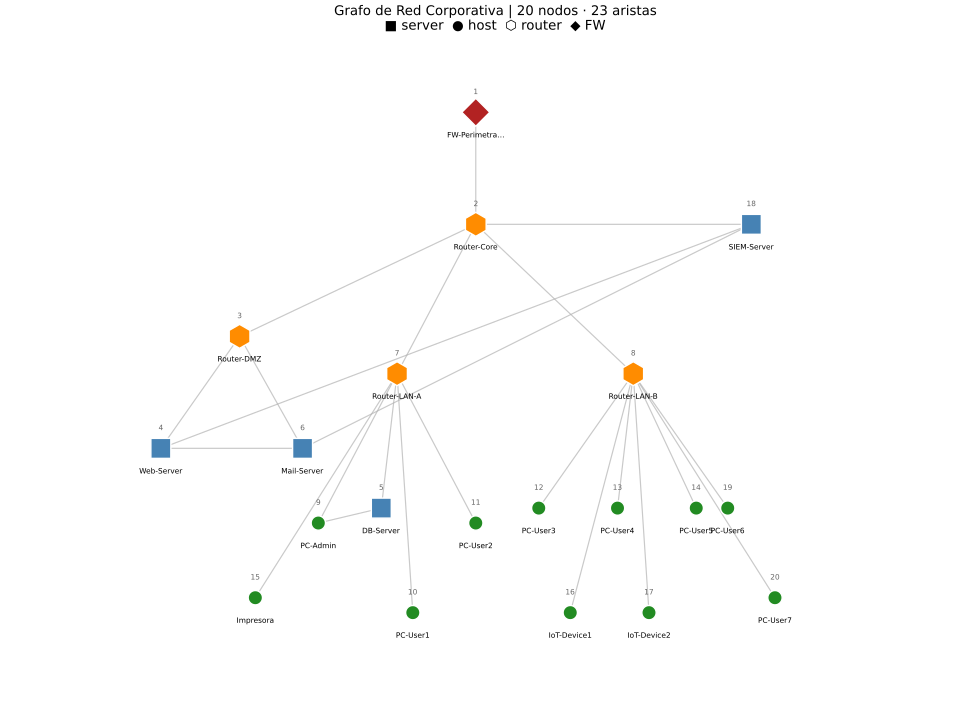
\includegraphics[width=0.75\linewidth,height=\textheight,keepaspectratio,alt={Grafo base de la red corporativa}]{grafo_red.png}
\caption{Grafo base de la red corporativa}
\end{figure}
\end{frame}

\subsection{Parte 2: metricas de
centralidad}\label{parte-2-metricas-de-centralidad}

\begin{frame}{Metricas calculadas}
\protect\phantomsection\label{metricas-calculadas}
{\def\LTcaptype{none} % do not increment counter
\begin{longtable}[]{@{}ll@{}}
\toprule\noalign{}
Metrica & Mide \\
\midrule\noalign{}
\endhead
Degree Centrality (DC) & Alcance local inmediato \\
Betweenness Centrality (BC) & Control de rutas minimas \\
Closeness Centrality (CC) & Rapidez para alcanzar la red \\
PageRank (PR) & Relevancia por estructura global \\
\bottomrule\noalign{}
\end{longtable}
}
\end{frame}

\begin{frame}{Hallazgo principal}
\protect\phantomsection\label{hallazgo-principal}
\begin{itemize}
\tightlist
\item
  \textbf{Router-LAN-B}: mayor intermediacion.
\item
  \textbf{Router-Core}: hub intersegmento (segundo lugar).
\item
  \textbf{FW-Perimetral}: relevancia operativa, baja topologica.
\end{itemize}

No basta contar conexiones --- importa cuantos caminos criticos dependen
del nodo.
\end{frame}

\subsection{Parte 2: grafo de
betweenness}\label{parte-2-grafo-de-betweenness}

\begin{frame}{Betweenness centrality}
\protect\phantomsection\label{betweenness-centrality}
\begin{figure}
\centering
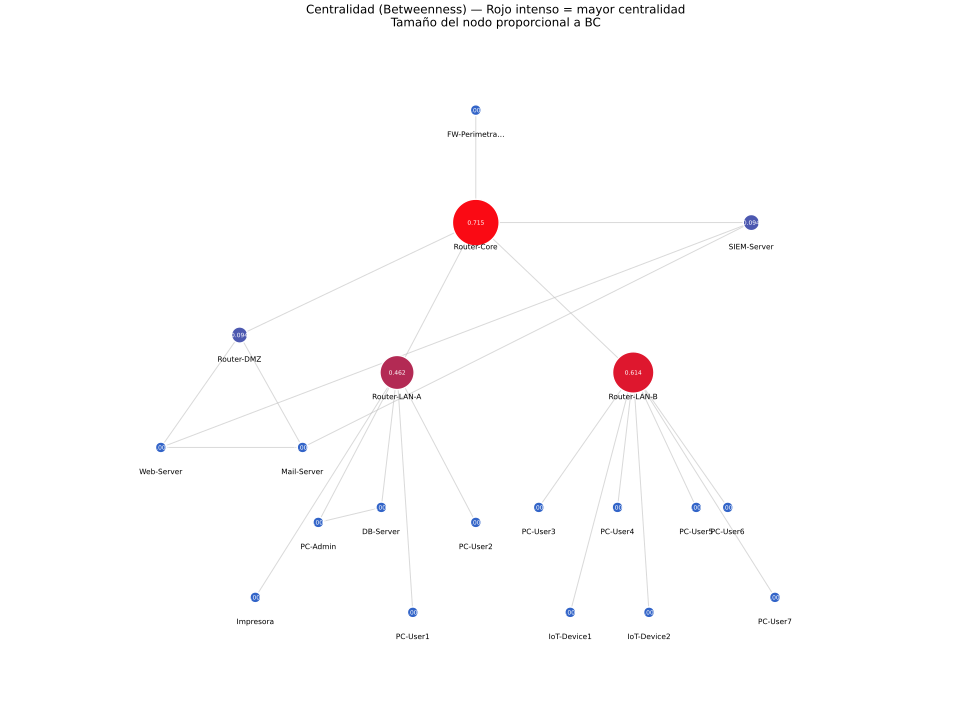
\includegraphics[width=0.85\linewidth,height=\textheight,keepaspectratio,alt={Grafo resaltando betweenness centrality}]{grafo_centralidad_bc.png}
\caption{Grafo resaltando betweenness centrality}
\end{figure}
\end{frame}

\subsection{Parte 2: comparacion de
centralidades}\label{parte-2-comparacion-de-centralidades}

\begin{frame}{Barras por metrica}
\protect\phantomsection\label{barras-por-metrica}
\begin{figure}
\centering
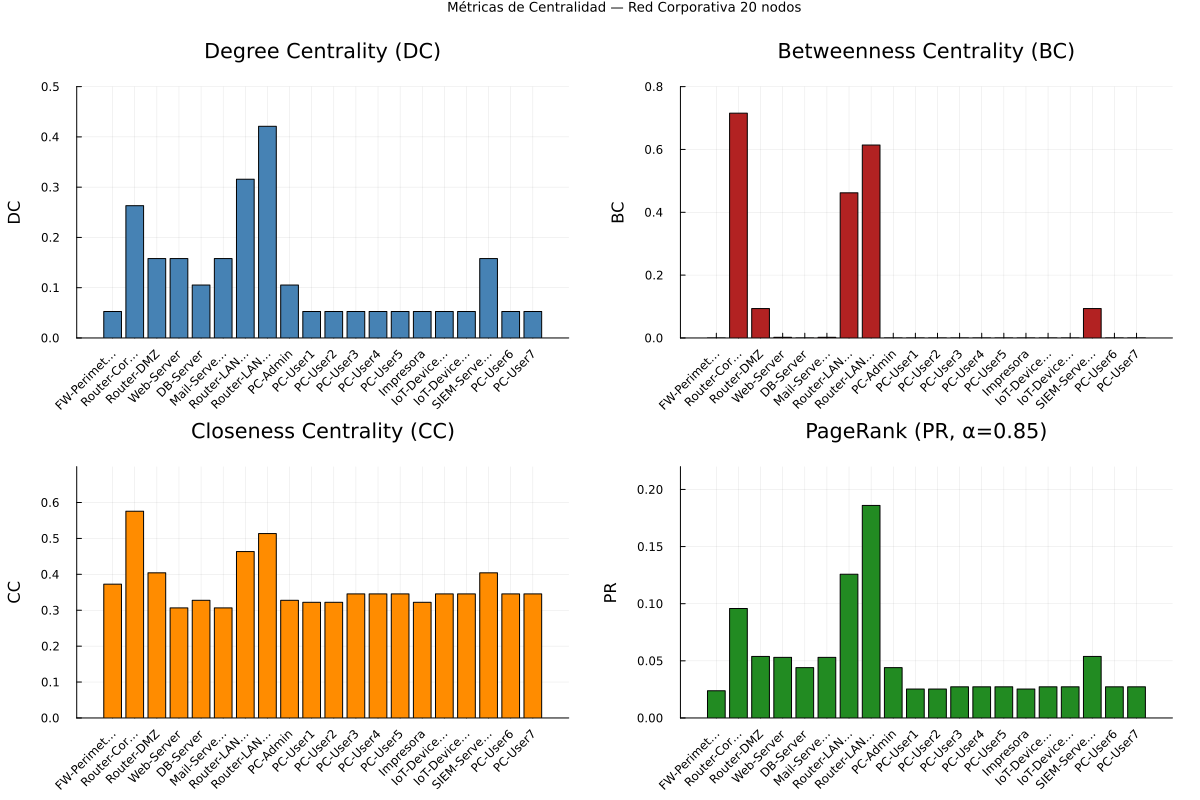
\includegraphics[width=0.85\linewidth,height=\textheight,keepaspectratio,alt={Comparacion de centralidades en barras}]{centralidad_barras.png}
\caption{Comparacion de centralidades en barras}
\end{figure}
\end{frame}

\subsection{Parte 3: deteccion de
anomalias}\label{parte-3-deteccion-de-anomalias}

\begin{frame}{Criterio estadistico}
\protect\phantomsection\label{criterio-estadistico}
\[score(v)=0.5\,BC(v)+0.3\,DC(v)+0.2\,PR(v) \quad z(v)=\frac{score(v)-\mu}{\sigma}\]

\begin{itemize}
\tightlist
\item
  Normalizar metricas, construir score ponderado, transformar a z-score.
\item
  \textbf{Umbral}: nodo anomalo si \(z > 1.5\).
\end{itemize}
\end{frame}

\begin{frame}{Nodos detectados}
\protect\phantomsection\label{nodos-detectados}
{\def\LTcaptype{none} % do not increment counter
\begin{longtable}[]{@{}ll@{}}
\toprule\noalign{}
Nodo & z-score \\
\midrule\noalign{}
\endhead
Router-LAN-B & 2.631 \\
Router-Core & 2.528 \\
Router-LAN-A & 1.791 \\
\bottomrule\noalign{}
\end{longtable}
}

Score compuesto reduce falsos positivos al combinar BC, DC y PR.
\end{frame}

\subsection{Parte 3: grafo de
anomalias}\label{parte-3-grafo-de-anomalias}

\begin{frame}{Nodos anomalos destacados}
\protect\phantomsection\label{nodos-anomalos-destacados}
\begin{figure}
\centering
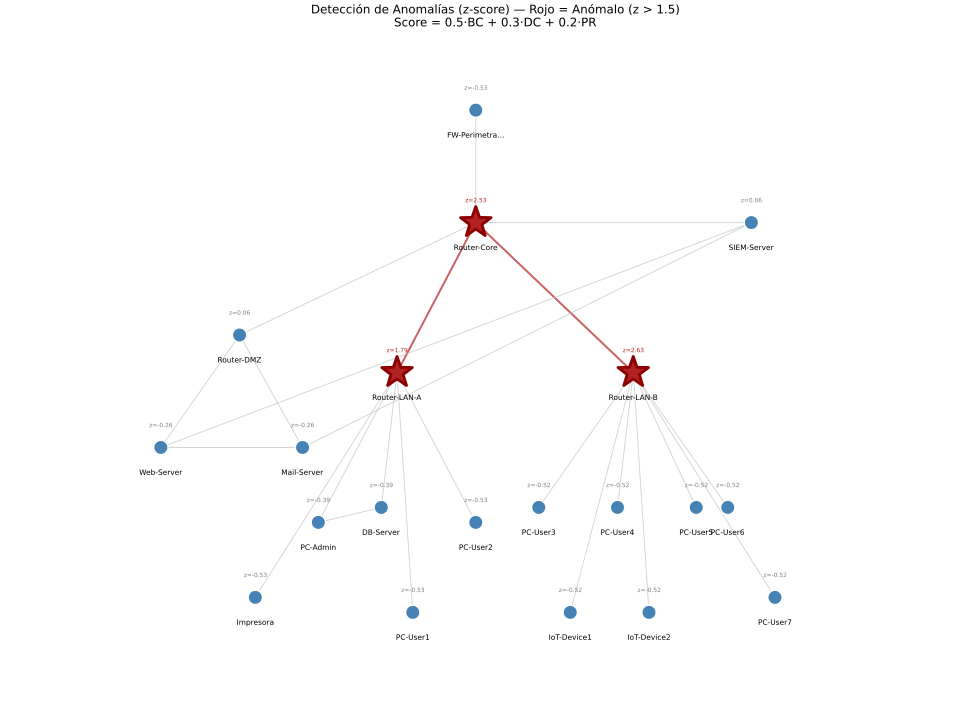
\includegraphics[width=0.85\linewidth,height=\textheight,keepaspectratio,alt={Grafo con nodos anomalos destacados}]{grafo_anomalias.png}
\caption{Grafo con nodos anomalos destacados}
\end{figure}
\end{frame}

\subsection{Parte 3: z-score por nodo}\label{parte-3-z-score-por-nodo}

\begin{frame}{Distribucion de z-scores}
\protect\phantomsection\label{distribucion-de-z-scores}
\begin{figure}
\centering
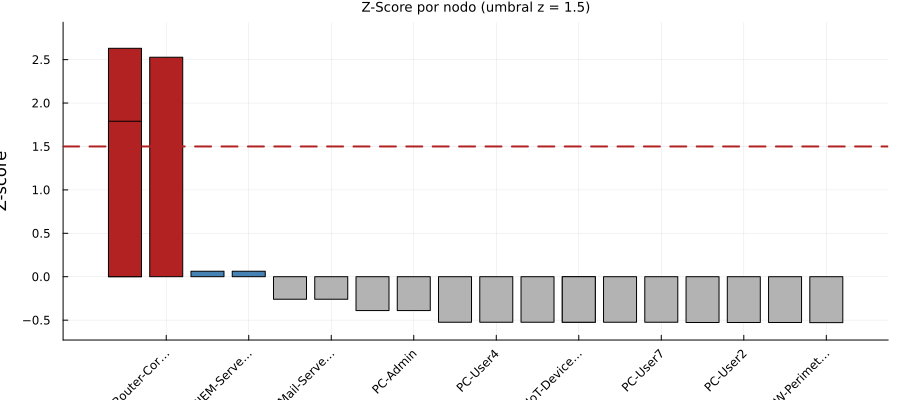
\includegraphics[width=0.85\linewidth,height=\textheight,keepaspectratio,alt={Barras de z-score por nodo}]{zscore_barras.png}
\caption{Barras de z-score por nodo}
\end{figure}
\end{frame}

\subsection{Parte 4: propagacion SIR}\label{parte-4-propagacion-sir}

\begin{frame}{Parametros y escenarios}
\protect\phantomsection\label{parametros-y-escenarios}
\begin{itemize}
\tightlist
\item
  Estados: Susceptible, Infectado, Recuperado.
\item
  \(\beta=0.3\), \(\gamma=0.1\), \(R_0=3\).
\item
  IoT-Device1 (periferia): tasa de ataque 5\%.
\item
  Router-Core (hub): tasa de ataque 50\%.
\end{itemize}

La posicion topologica condiciona mas el impacto que \(R_0\).
\end{frame}

\subsection{Parte 4: curvas SIR}\label{parte-4-curvas-sir}

\begin{frame}{Comparacion de curvas}
\protect\phantomsection\label{comparacion-de-curvas}
\begin{figure}
\centering
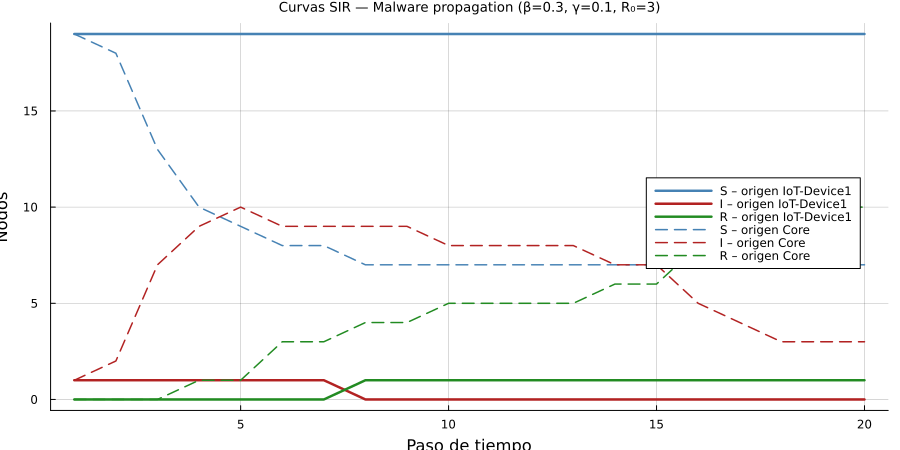
\includegraphics[width=0.85\linewidth,height=\textheight,keepaspectratio,alt={Comparacion de curvas SIR}]{sir_comparacion.png}
\caption{Comparacion de curvas SIR}
\end{figure}
\end{frame}

\subsection{Parte 4: sensibilidad}\label{parte-4-sensibilidad}

\begin{frame}{Barrido de \(\beta\) desde nodo periferico}
\protect\phantomsection\label{barrido-de-beta-desde-nodo-periferico}
\begin{itemize}
\tightlist
\item
  \(\beta=0.1, 0.2, 0.3\): sin epidemia desde IoT-Device1.
\item
  \(\beta=0.5\): brote escapa de la periferia.
\item
  Topologia actua como barrera natural en nodos hoja.
\end{itemize}
\end{frame}

\subsection{\texorpdfstring{Parte 4: barrido de
\(\beta\)}{Parte 4: barrido de \textbackslash beta}}\label{parte-4-barrido-de-beta}

\begin{frame}{Resultado del barrido}
\protect\phantomsection\label{resultado-del-barrido}
\begin{figure}
\centering
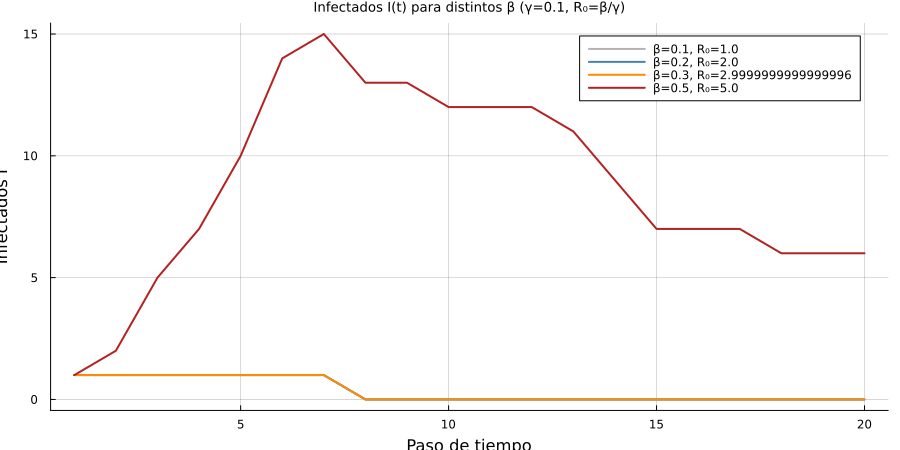
\includegraphics[width=0.85\linewidth,height=\textheight,keepaspectratio,alt={Barrido de beta en la simulacion SIR}]{sir_betas.png}
\caption{Barrido de beta en la simulacion SIR}
\end{figure}
\end{frame}

\subsection{Parte 4: cuarentena}\label{parte-4-cuarentena}

\begin{frame}{Efecto de aislamiento temprano}
\protect\phantomsection\label{efecto-de-aislamiento-temprano}
\begin{itemize}
\tightlist
\item
  Aislar nodo central reduce nodos alcanzables.
\item
  Interrumpe corredores topologicos de propagacion.
\end{itemize}
\end{frame}

\subsection{Parte 4: impacto de
cuarentena}\label{parte-4-impacto-de-cuarentena}

\begin{frame}{Resultado}
\protect\phantomsection\label{resultado}
\begin{figure}
\centering
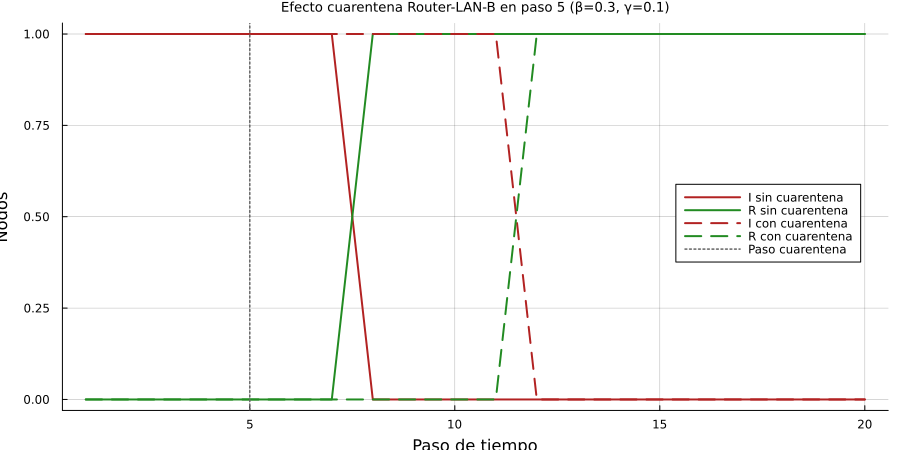
\includegraphics[width=0.85\linewidth,height=\textheight,keepaspectratio,alt={Impacto de una cuarentena temprana}]{sir_cuarentena.png}
\caption{Impacto de una cuarentena temprana}
\end{figure}
\end{frame}

\subsection{Parte 5: resiliencia de la
red}\label{parte-5-resiliencia-de-la-red}

\begin{frame}{Metricas estructurales}
\protect\phantomsection\label{metricas-estructurales}
{\def\LTcaptype{none} % do not increment counter
\begin{longtable}[]{@{}ll@{}}
\toprule\noalign{}
Metrica & Valor \\
\midrule\noalign{}
\endhead
Nodos de articulacion & 3 \\
Puentes & 13 \\
Conectividad \(\kappa\) & 1 \\
\bottomrule\noalign{}
\end{longtable}
}

\begin{itemize}
\tightlist
\item
  Red no 2-conexa.
\item
  Multiples enlaces sin redundancia.
\item
  Puntos unicos de fallo en backbone y distribucion.
\end{itemize}
\end{frame}

\begin{frame}{Nodo mas critico}
\protect\phantomsection\label{nodo-mas-critico}
\textbf{Router-Core}: su falla fragmenta la red y aisla segmentos
completos.
\end{frame}

\subsection{Parte 5: articulaciones y
puentes}\label{parte-5-articulaciones-y-puentes}

\begin{frame}{Grafo de resiliencia}
\protect\phantomsection\label{grafo-de-resiliencia}
\begin{figure}
\centering
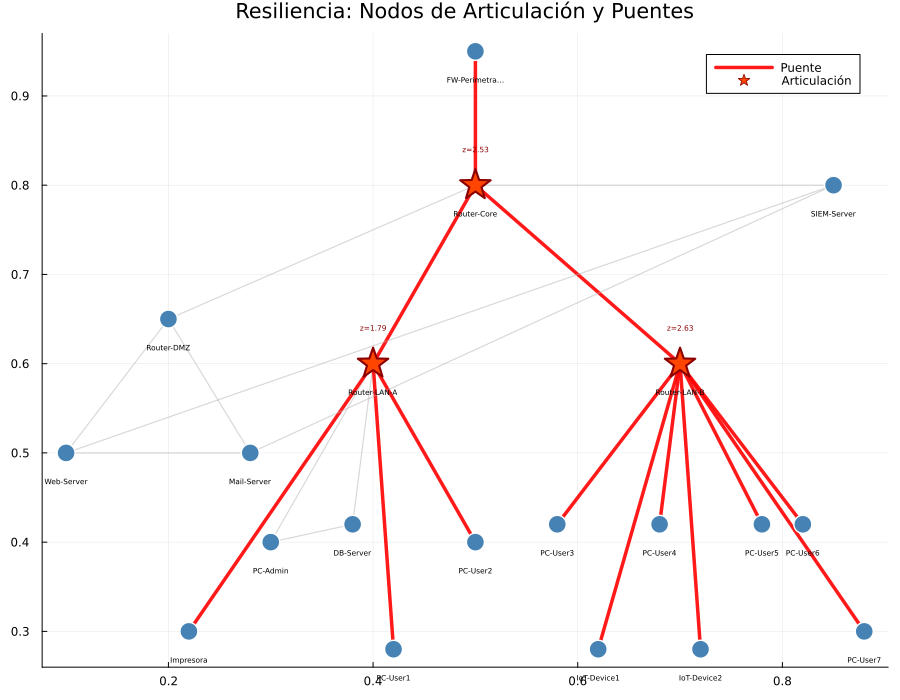
\includegraphics[width=0.85\linewidth,height=\textheight,keepaspectratio,alt={Grafo con articulaciones y puentes}]{resiliencia_grafo.png}
\caption{Grafo con articulaciones y puentes}
\end{figure}
\end{frame}

\subsection{Parte 5: impacto por
eliminacion}\label{parte-5-impacto-por-eliminacion}

\begin{frame}{Degradacion ante fallos dirigidos}
\protect\phantomsection\label{degradacion-ante-fallos-dirigidos}
\begin{figure}
\centering
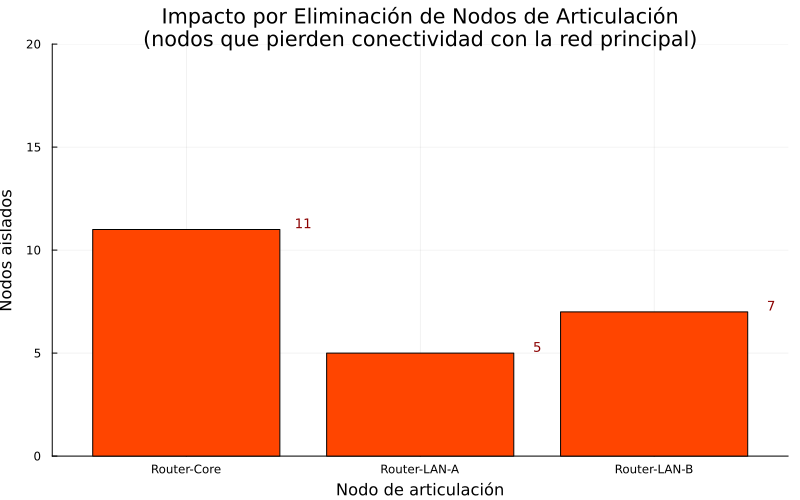
\includegraphics[width=0.85\linewidth,height=\textheight,keepaspectratio,alt={Impacto por eliminacion de nodos criticos}]{resiliencia_impacto.png}
\caption{Impacto por eliminacion de nodos criticos}
\end{figure}
\end{frame}

\subsection{Hardening propuesto}\label{hardening-propuesto}

\begin{frame}{Recomendaciones priorizadas}
\protect\phantomsection\label{recomendaciones-priorizadas}
{\def\LTcaptype{none} % do not increment counter
\begin{longtable}[]{@{}
  >{\raggedright\arraybackslash}p{(\linewidth - 4\tabcolsep) * \real{0.3333}}
  >{\raggedright\arraybackslash}p{(\linewidth - 4\tabcolsep) * \real{0.3333}}
  >{\raggedright\arraybackslash}p{(\linewidth - 4\tabcolsep) * \real{0.3333}}@{}}
\toprule\noalign{}
\begin{minipage}[b]{\linewidth}\raggedright
Prioridad
\end{minipage} & \begin{minipage}[b]{\linewidth}\raggedright
Medida
\end{minipage} & \begin{minipage}[b]{\linewidth}\raggedright
Efecto
\end{minipage} \\
\midrule\noalign{}
\endhead
1 & Router-Core redundante & \(\kappa\): 1 \(\to\) 2 \\
2 & Enlace directo LAN-A \(\leftrightarrow\) LAN-B & Menos puentes
criticos \\
3 & Segunda conexion al firewall & Eliminar SPOF perimetral \\
4 & Enlace SIEM-Server a Router-LAN-A & Resiliencia de monitoreo \\
\bottomrule\noalign{}
\end{longtable}
}
\end{frame}

\begin{frame}{Idea central}
\protect\phantomsection\label{idea-central}
No agregar enlaces indiscriminadamente --- incorporar rutas alternativas
donde hoy existe dependencia de un unico nodo o arista.
\end{frame}

\subsection{Desafio extra: IoT-23}\label{desafio-extra-iot-23}

\begin{frame}{Datos analizados}
\protect\phantomsection\label{datos-analizados}
{\def\LTcaptype{none} % do not increment counter
\begin{longtable}[]{@{}lll@{}}
\toprule\noalign{}
Captura & Tipo & Lineas \\
\midrule\noalign{}
\endhead
Capture-1-1 & Mirai & 150 001 \\
Capture-3-1 & Mirai variante & 150 001 \\
Capture-42-1 & C\&C FileDownload & 4 001 \\
\bottomrule\noalign{}
\end{longtable}
}
\end{frame}

\begin{frame}[fragile]{Metodologia}
\protect\phantomsection\label{metodologia}
\begin{enumerate}
\tightlist
\item
  Grafo dirigido IP \(\rightarrow\) IP desde \texttt{conn.log.labeled}.
\item
  Score botnet por IP: \(\%{}Mal\), DC, BC, \(Ports_{norm}\).
\item
  Marcacion por z-score y validacion contra \texttt{label}.
\end{enumerate}

\[score_{botnet}(v)=0.35\,\%{}Mal+0.25\,DC+0.20\,BC+0.20\,Ports_{norm}\]
\end{frame}

\subsection{Desafio extra: resultados}\label{desafio-extra-resultados}

\begin{frame}{IPs detectadas y desempeno}
\protect\phantomsection\label{ips-detectadas-y-desempeno}
\begin{itemize}
\tightlist
\item
  \textbf{192.168.100.103} en Capture-1-1 --- F1=1.000, \(z>8\).
\item
  \textbf{192.168.2.5} en Capture-3-1 --- F1=1.000, \(z>8\).
\item
  Variable clave: \(\%{}Mal\) + \(Ports_{norm}\) juntos.
\end{itemize}
\end{frame}

\subsection{Desafio extra: comparacion de
capturas}\label{desafio-extra-comparacion-de-capturas}

\begin{frame}{Severidad por captura}
\protect\phantomsection\label{severidad-por-captura}
\begin{figure}
\centering
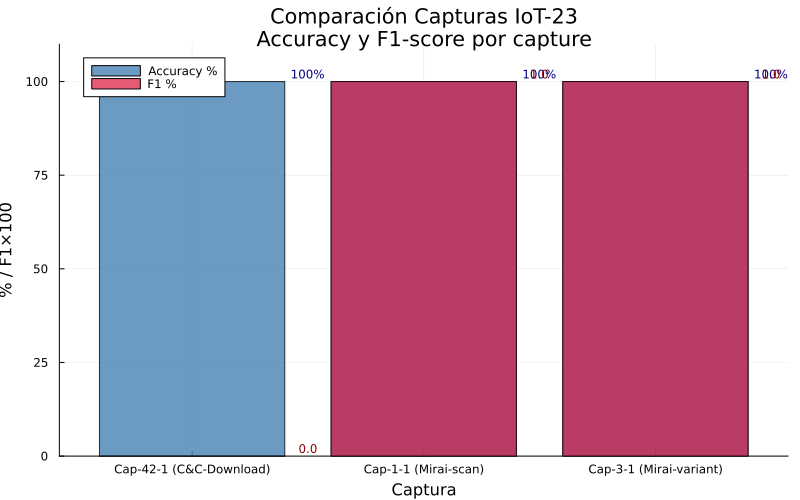
\includegraphics[width=0.85\linewidth,height=\textheight,keepaspectratio,alt={Comparacion entre capturas IoT-23}]{botnet_comparacion.png}
\caption{Comparacion entre capturas IoT-23}
\end{figure}
\end{frame}

\subsection{Desafio extra: z-score
Mirai}\label{desafio-extra-z-score-mirai}

\begin{frame}{Deteccion por IP}
\protect\phantomsection\label{deteccion-por-ip}
\begin{figure}
\centering
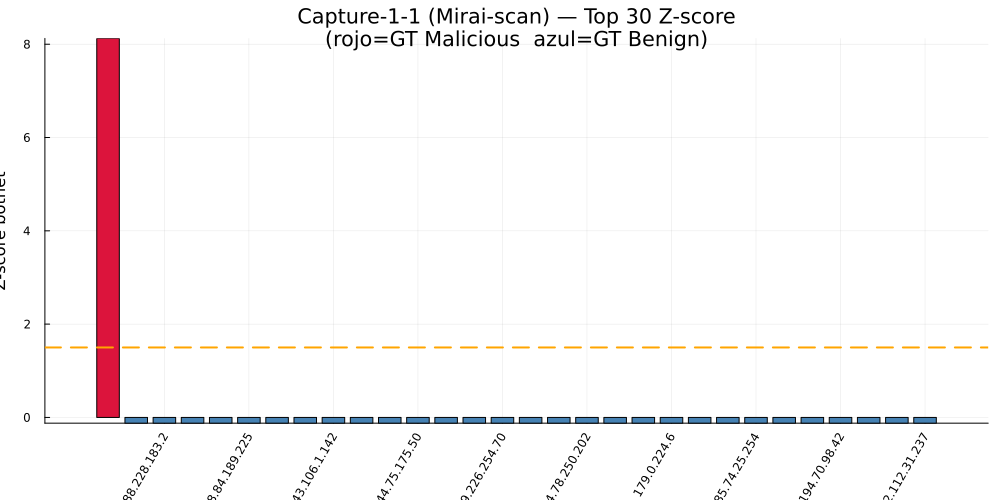
\includegraphics[width=0.85\linewidth,height=\textheight,keepaspectratio,alt={Z-score de deteccion para Mirai}]{botnet_Capture11_Miraiscan_zscore.png}
\caption{Z-score de deteccion para Mirai}
\end{figure}
\end{frame}

\subsection{Desafio extra: matriz de
confusion}\label{desafio-extra-matriz-de-confusion}

\begin{frame}{Validacion multicaptura}
\protect\phantomsection\label{validacion-multicaptura}
\begin{figure}
\centering
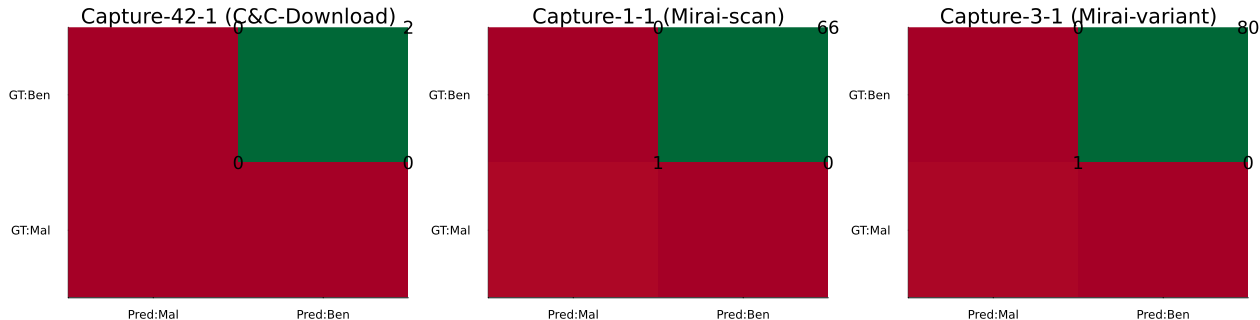
\includegraphics[width=0.85\linewidth,height=\textheight,keepaspectratio,alt={Matriz de confusion multicaptura}]{botnet_confusion_multi.png}
\caption{Matriz de confusion multicaptura}
\end{figure}
\end{frame}

\subsection{Integracion de resultados}\label{integracion-de-resultados}

\begin{frame}{Convergencia entre metodos}
\protect\phantomsection\label{convergencia-entre-metodos}
\begin{itemize}
\tightlist
\item
  Nodos anomalos (Parte 3) coinciden con articulaciones (Parte 5).
\item
  Router-Core: mayor anomalia, mejor punto de inicio para brote severo
  (Parte 4).
\item
  Metodologia detecta criticidad estructural y riesgo operativo
  simultaneamente.
\end{itemize}
\end{frame}

\begin{frame}{Lectura final}
\protect\phantomsection\label{lectura-final}
Score compuesto de centralidad = predictor robusto de criticidad. Su
extension a trafico real detecta botnets con alta precision.
\end{frame}

\subsection{Conclusiones}\label{conclusiones}

\begin{frame}{Conclusiones principales}
\protect\phantomsection\label{conclusiones-principales}
\begin{enumerate}
\tightlist
\item
  Red corporativa funcional, pero fragil ante fallos dirigidos.
\item
  Centralidad identifica activos cuya perdida rompe conectividad.
\item
  Propagacion depende fuertemente de posicion del nodo inicial.
\item
  Resiliencia mejora eliminando SPOF e incrementando redundancia.
\item
  Metodologia validada en IoT-23 con F1=1.0 para Mirai.
\end{enumerate}
\end{frame}

\begin{frame}{Mensaje final}
\protect\phantomsection\label{mensaje-final}
La integracion de teoria de grafos, simulacion epidemiologica y analisis
estadistico ofrece un marco coherente para priorizar defensa, deteccion
y hardening en redes reales.
\end{frame}
